\documentclass[10pt,twocolumn]{article}

\usepackage[small,compact]{titlesec} %http://gurmeet.net/computer-science/latex-tips-n-tricks-for-conference-papers/
\usepackage{microtype} % Make the font and alignment look cleaner
\usepackage{graphicx}

% For \overset, etc.
\usepackage{amsmath}
\usepackage{cancel}

%%%%%%%%%%%%%%%%%%%%%%%%%%%%%% Margins
\setlength{\columnsep}{0.25in}
\usepackage[top=0.8in,bottom=0.8in,left=0.5in,right=0.5in]{geometry}




%==================================================================================================
%   MATH MACROS
\newcommand{\mabs}[1]{\ensuremath{  \left| #1 \right|  }}
\newcommand{\argmax}[2]{\ensuremath{   \underset{#1}{\operatorname{argmax}} \left\{ #2 \right\}  }} 

\newcommand{\prb}[1]{\ensuremath{  \mathrm{Pr}\left\{ #1 \right\}  }}
\newcommand{\Elin}[1]{\ensuremath{     \mathrm{E}\left[ #1 \right]   }}

\newcommand{\tridefeq}{\ensuremath{  \,{\overset{\triangle}{=}}\;   }}

\newcommand{\normrv}[2]{\ensuremath{          \mathcal{N}\left(#1,#2\right)    }}

\newcommand{\ind}[1]{\ensuremath{  \pmb{\mathtt{1}}\left\{ #1 \right\}  }}

%==================================================================================================

\begin{document}


 \twocolumn[%
 \centerline{\Large \bf Bayesian Skill Ranking} %% Paper title

 \medskip

 \centerline{\bf Leland Chen, Joseph Huang, Ryan Thompson}      %% Author name(s)
 \centerline{\today}

 \bigskip
 ]

% ==============================================================================
% ==============================================================================

\section{Introduction}

  Template

% ==============================================================================
% ==============================================================================

\section{Related Work}

Let's talk about~\cite{herbrich2007trueskilltm}~and~\cite{coulom2008whole} and then just follow the citations that those guys make to introduce the general challenges and state-of-the art.

Basketball brings two key challenges to the field of Bayesian Skill estimation.
\begin{itemize}
\item Results are not binary Win/Lose outcomes.
\item Results are influenced by the skill differential of more than two players.
\end{itemize}


% ==============================================================================
% ==============================================================================

\section{Method}
\subsection{Traditional Networks}

We model the result of each possession as an independent and identically distributed random variable, \emph{Result}.
An NBA roster has 12 players, but only five of them are on the court for a given team during any single posession.

To reduce noise, we ignore ``garbage time'' posessions. To simplify the model we ignore possessions that end in a time-out.

We begin with a very basic model that follows traditional ``skill ranking'' in the sense that each player has an unobserved (or parameterized) skill that has some distribution, and using inference (or parameter estimation) we can determine the value of each player's skill.
In this network, we decided each player would have a hidden offsensive and defensive skill value, shared across possessions:
\begin{center}
	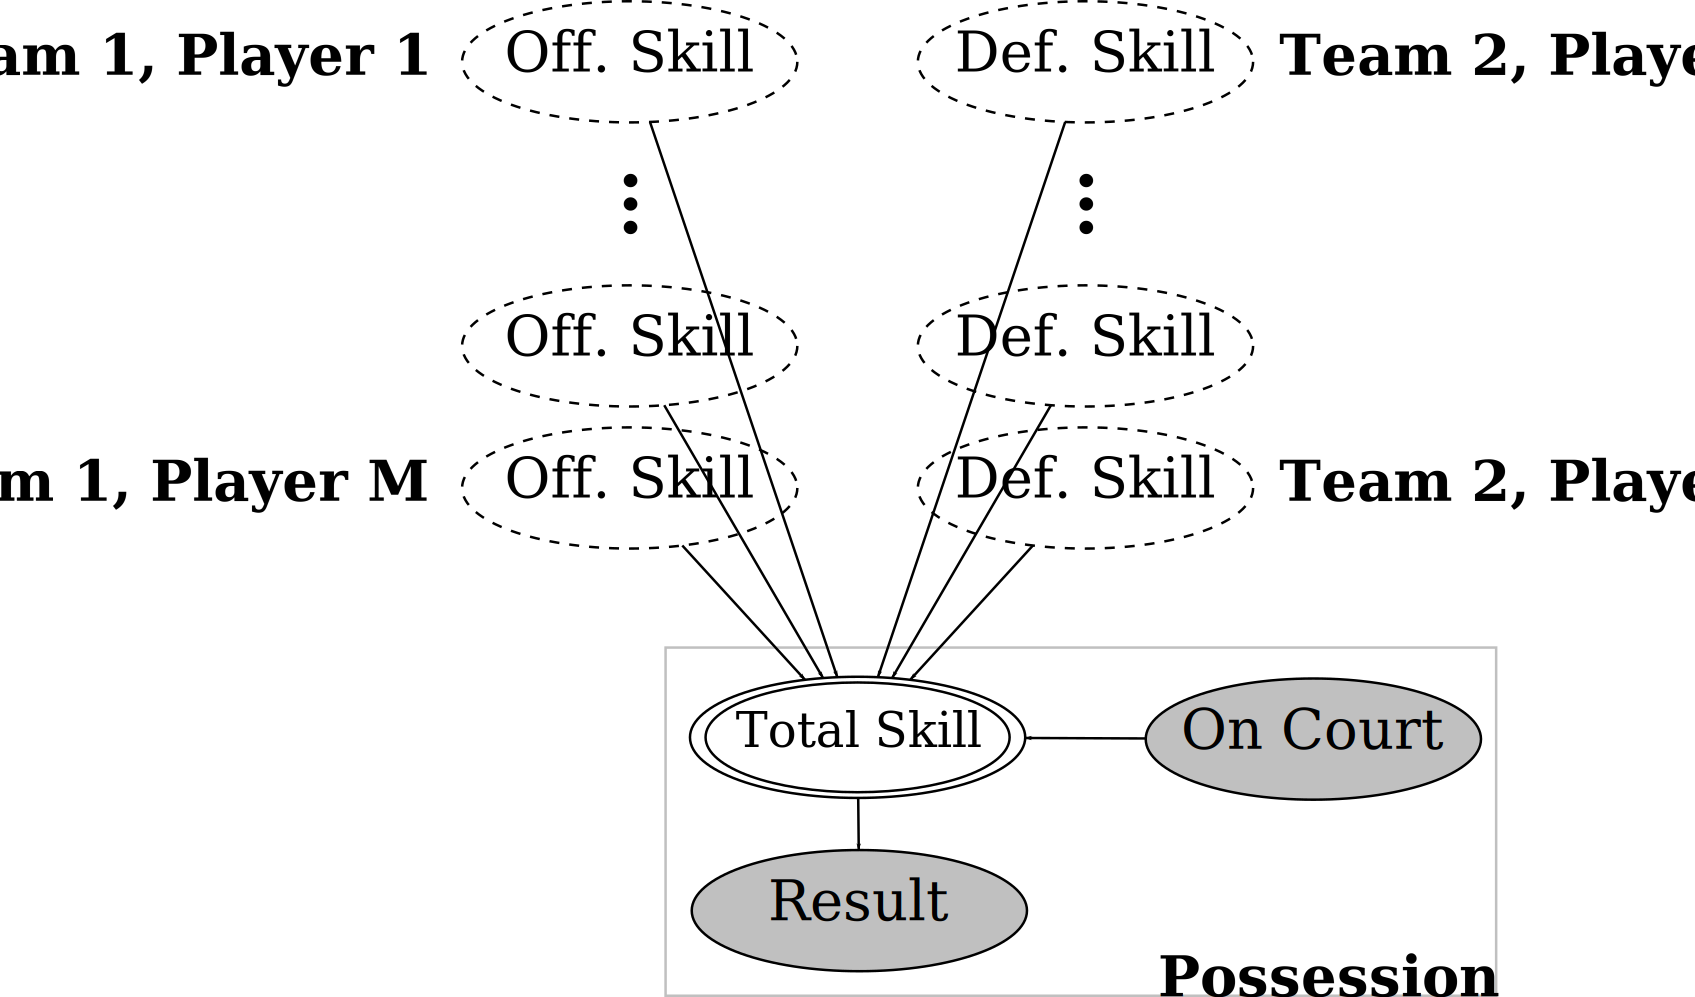
\includegraphics[width=0.90\linewidth]{figures/network}
\end{center}
These skills would contribute deterministically in some way to an ``effective'' total skill differential between the two teams, and then the \emph{Result} variable would be one of four outcomes:
\begin{itemize}
\item $R=0$ Offensive Team Scores nothing, change of possession (e.g. turnover, defensive rebound, etc.)
\item $R=1$ Offensive Team Scores 1 point
\item $R=2$ Offensive Team Scores 2 points
\item $R=3$ Offensive Team Scores 3 points
\end{itemize}

The \emph{On Court} random variable ``multiplexes'' between those players that are on the court and those that are not.

% ==============================================================================
\subsection{Issues}
\label{sec:badnetwork}
These traditional models~\cite{herbrich2007trueskilltm} have difficulty capturing the proper causalities when Results can have multinomial-valued outcomes.
For example, regardless of the parameterization of the \emph{Results} CPD, both $\prb{ R = 2}$ and $\prb{R= 3}$ would depend on the same skills of the same players.
The relative distribution of outcomes $\prb{R = 2}$ vs. $\prb{R = 3}$ would be shared across all ``units'' (i.e. all combinations of \emph{On Court} assignments).

In reality, a team that scores $R=3$ half the time and $R=1$ half the time is just as good as a team that scores $R=2$ all the time.
However, any traditional Win/Lose model will unfairly penalize the likelihood of one of these teams over the other and leads to under-fitting.
This might suggest that we have a random variable that represents $\Elin{\mathrm points scored}$, but this doesn't pass the clarity test.


% TODO(jdhuang): Modular in Win_i would be very meaningful

Secondly, there is a lot of value in being able to compare with the state-of-the-art in the Win/Lose based Bayesian Skill Ranking literature.
Specifically, there is common debate over logistic vs. Gaussian skill/performance distributions and we wish to be sensitive to that conversation in this project.
Having a multinomial outcome makes it difficult to directly compare logistic vs. Gaussian in the standard skill/performance framework because there is no consensus in the literature about how to extend these models just to support ties~\cite{hunter2004mm}, let alone general multinomial outcomes.

% ==============================================================================
\subsection{Proposed Network}

To address some of the shortcomings discussed in {\bf Section~\ref{sec:badnetwork}}, we propose the following:
\begin{center}
	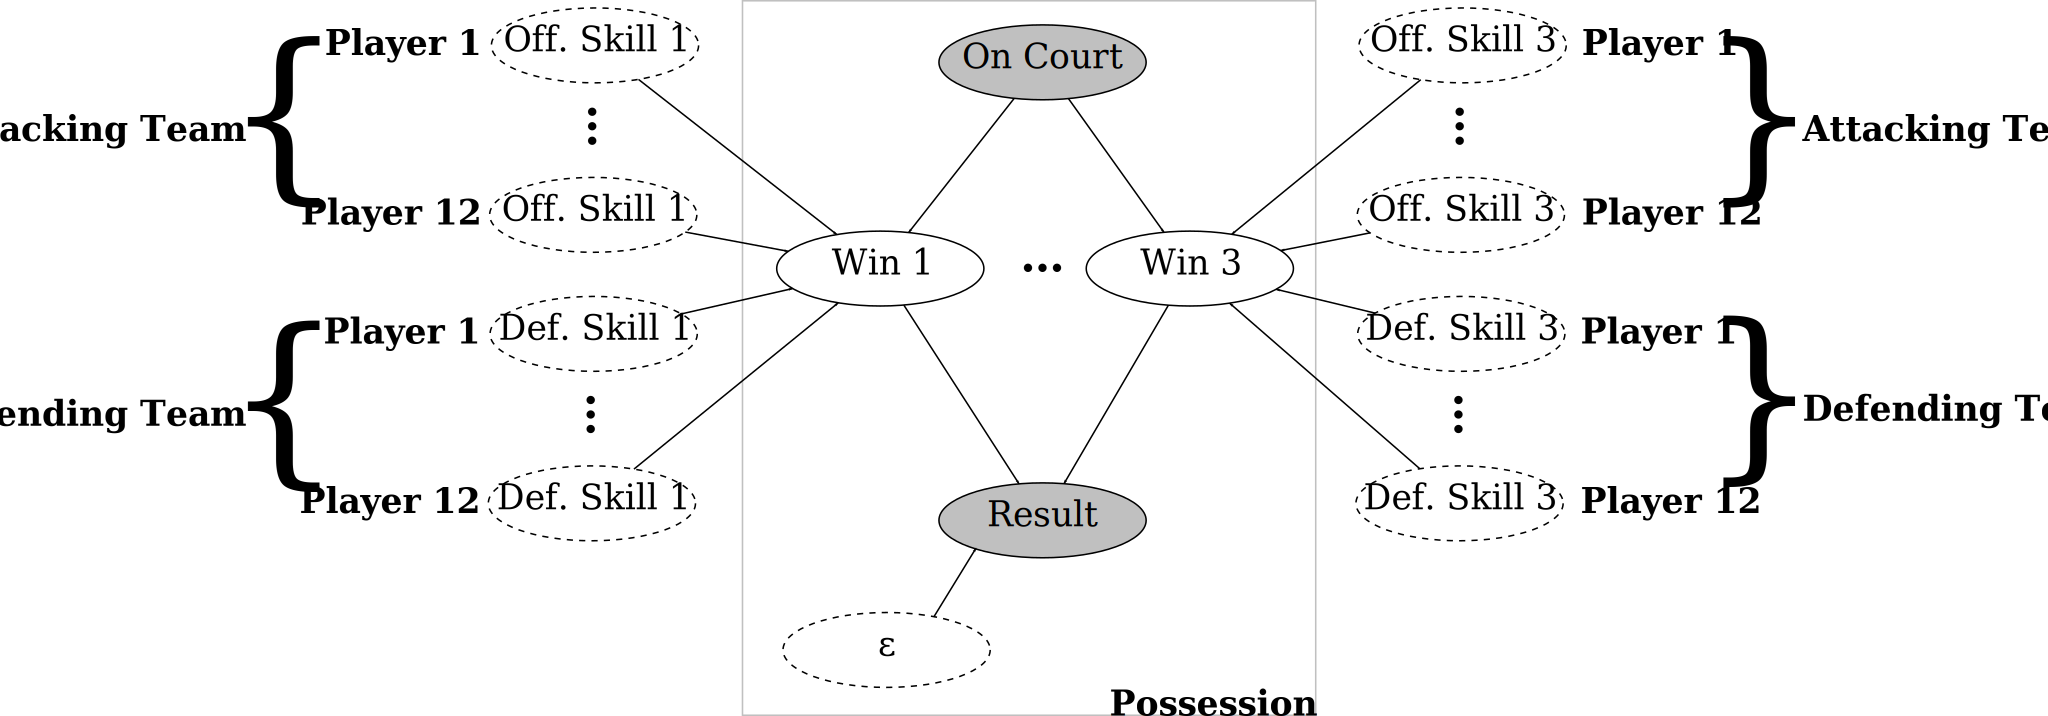
\includegraphics[width=1.05\linewidth]{figures/newnetwork}
\end{center}

In this network, each player is represented by three skill parameters:
\begin{enumerate}
\item Skill 1: Ability to score (or defend against) one-point opportunities
\item Skill 2: Ability to score (or defend against) two-point opportunities
\item Skill 3: Ability to score (or defend against) three-point opportunities
\end{enumerate}

For notational convenience, let
\[
A\left(\mathrm{Skills}\right) \tridefeq \exp \left( \sum_i \textrm{Off. Team, Player i Off. Skill } k \right)
%\quad, \quad \quad
\]%
\[
B\left(\mathrm{Skills}\right) \tridefeq  \exp \left( \sum_i \textrm{Def. Team, Player i Def. Skill } k \right)
\]%
where
\begin{align*}
\vec \theta_k =& \left\{\textrm{Off. Team, Player i Off. Skill } k\right\}_k
\\             &\cup \left\{\textrm{Def. Team, Player i Def. Skill } k\right\}_k
\end{align*}%

On each possession, there are three binary hidden random variables defined by a probability function with parameters that we will learn. In particular, each of the ``Win'' random variables depends on the corresponding skills of players on court as input (which are learned):
\begin{enumerate}
\item \emph{Win 1}: True if there was a {\bf guaranteed opportunity} to score one point at some point during the possession.
\item \emph{Win 2}: True if there was a {\bf guaranteed opportunity} to score two points at some point during the possession.
\item \emph{Win 3}: True if there was a {\bf guaranteed opportunity} to score three points at some point during the possession.
\end{enumerate}
Note: The term ``opportunity'' is not intended in the typical basketball sense, where it often means ``the opportunity to take a shot''.


Each of the \emph{Win k} events has a CPD parameterized by $\vec \theta_k$ (whose values we will learn during training), which depends on the skills of the players.
In the basic model of player skills, the skill of a five-man team is the sum of the skills of its players.

For example, in a Bradley-Terry model, we might have:
\[
\prb{\mathrm{Win}_k = \mathbf{True} \mid \mathrm{Skills} } = \frac{ A\left(\mathrm{Skills}\right) } { A\left(\mathrm{Skills}\right) + B\left(\mathrm{Skills}\right) }
\]%
Alternatively, in a Thurstone Case V model, we might have:
\[
\prb{\mathrm{Win}_k = \mathbf{True} \mid \mathrm{Skills} } = \Phi\left( A - B \right)
\]%

For notational convenience, we will write $W_k = w_k^1$ for $\mathrm{Win}_k = \mathbf{True}$, and $W_k = w_k^0$ when {\bf False}.

To understand the relationship between $\left\{Win\right\}$ and $Result$, let's go through an example.
Imagine that for a particular five-man unit, the $\theta$ are known and the resulting probabilities are:
\begin{align*}
\prb{W_1=w_1^1} = 1\% \quad&, \quad\quad \prb{W_1=w_1^0} = 99\%
\\
\prb{W_2=w_2^1} = 25\% \quad&, \quad\quad \prb{W_2=w_2^0} = 75\%
\\
\prb{W_3=w_3^1} = 30\% \quad&, \quad\quad \prb{W_3=w_3^0} = 70\%
\end{align*}%
This means, on each possession
\begin{itemize}
\item the offensive team has a $30\%$ probability of scoring 3 points (i.e. $R=r^3$ with 30\% probability)
\item the offensive team has a $\left(100\% - 30\%\right) \times 25\%$ probability of scoring 2 points (i.e. $\prb{R=r^2}=17.5\%$)
\item the offensive team has a $70\% \times 75\% \times 1\%$ probability of scoring 1 point (i.e. $\prb{R=r^1}=0.525\%$)
\item the offensive team has a $51.975\%$ chance of scoring 0 points
\end{itemize}

Essentially, \emph{Result} simply selects the highest-scoring decision available during the possession.
If \emph{Win 3} is true, \emph{Result} is 3; If \emph{Win 3} is false but \emph{Win 2} is true, \emph{Result} is 2; etc.

\emph{Result} can be specified with either a tree-CPD or table-CPD, but it has the following probabilities.

\begin{tabular}{ r|c c c c|}
$R|W_1,W_2,W_3$ & $R=r^0$ & $R=r^1$ & $R=r^2$ & $R=r^3$ \\  \hline
$w^1_3 w^1_2 w^1_1$ & $\varepsilon$ &  $\varepsilon$ &  $\varepsilon$ & $(1 - 3 \varepsilon)$ \\ \hline
$w^1_3 w^1_2 w^0_1$ & $\varepsilon$ &  $\varepsilon$ &  $\varepsilon$ & $(1 - 3 \varepsilon)$ \\ \hline
$w^1_3 w^0_2 w^1_1$ & $\varepsilon$ &  $\varepsilon$ &  $\varepsilon$ & $(1 - 3 \varepsilon)$ \\ \hline
$w^1_3 w^0_2 w^0_1$ & $\varepsilon$ &  $\varepsilon$ &  $\varepsilon$ & $(1 - 3 \varepsilon)$ \\ \hline
$w^0_3 w^1_2 w^1_1$ & $\varepsilon$ &  $\varepsilon$ &  $(1 - 3 \varepsilon)$ & $\varepsilon$ \\ \hline
$w^0_3 w^1_2 w^0_1$ & $\varepsilon$ &  $\varepsilon$ &  $(1 - 3 \varepsilon)$ & $\varepsilon$ \\ \hline
$w^0_3 w^0_2 w^1_1$ & $\varepsilon$ & $(1 - 3 \varepsilon)$   & $\varepsilon$ & $\varepsilon$ \\ \hline
$w^0_3 w^0_2 w^0_1$ & $(1 - 3 \varepsilon)$ & $\varepsilon$   & $\varepsilon$ & $\varepsilon$ \\ \hline
\end{tabular}


The single parameter $\varepsilon$ is inspired by the noisy-max and essentially indicates unmodelled errors (e.g. offensive or defensive mistakes).
The better our model fits the actual flow of the game, the smaller $\varepsilon$ should be.


% ==============================================================================
% ==============================================================================

\section{Implemention}

Maximum Likelihood starts with:
\begin{align*}
L &= \prod_{\mathcal{D}} \prb{\mathcal{D} \mid \vec \theta_1,\vec \theta_2,\vec \theta_3, \varepsilon}
\\ &=
\prod_{\mathcal{D}}
\sum_{\substack{w_1 \in \operatorname{Val}\left(W_1\right) \\ w_2 \in \operatorname{Val}\left(W_2\right) \\ w_3 \in \operatorname{Val}\left(W_3\right)}}
\\ & \quad \quad \prb{R = \mathcal{D}_r, W_1 = w_1, W_2 = w_2, W_3 = w_3 \mid \vec \theta_1,\vec \theta_2,\vec \theta_3, \varepsilon}
\end{align*}%
\begin{align*}
= \prod_{\mathcal{D}}
 & \sum_{\substack{w_1 \in \operatorname{Val}\left(W_1\right) \\ w_2 \in \operatorname{Val}\left(W_2\right) \\ w_3 \in \operatorname{Val}\left(W_3\right)}}
\\ & \prb{R = \mathcal{D}_r \mid W_1 = w_1, W_2 = w_2, W_3 = w_3, \cancel{ \vec \theta_1,\vec \theta_2,\vec \theta_3}, \varepsilon}
\\ & \prb{W_1 = w_1 \mid \vec \theta_1, \cancel{\vec \theta_2,\vec \theta_3, \varepsilon}}
\\ & \prb{W_2 = w_2 \mid \vec \theta_2, \cancel{\vec \theta_1,\vec \theta_3, \varepsilon}}
\\ & \prb{W_3 = w_3 \mid \vec \theta_3, \cancel{\vec \theta_1,\vec \theta_2, \varepsilon}}
\end{align*}%
%which provides global decomposition allowing us to log-maximize each section of the network separately:
%\begin{align*}
%L = & \left( \prod_{\mathcal{D}} \sum_{w_1,w_2,w_3} \prb{R = \mathcal{D}_r \mid W_1 = w_1, W_2 = w_2, W_3 = w_3, \varepsilon} \right)
%\\ & \left( \prod_{\mathcal{D}} \sum_{w_1} \prb{W_1 = w_1 \mid \vec \theta_1} \right)
%\\ & \left( \prod_{\mathcal{D}} \sum_{w_2} \prb{W_2 = w_2 \mid \vec \theta_2} \right)
%\\ & \left( \prod_{\mathcal{D}} \sum_{w_3} \prb{W_3 = w_3 \mid \vec \theta_3} \right)
%\end{align*}%

In the M-step, we assume $\mathcal{D}$ has observed $W_1 = \mathcal{D}_1$, $W_2= \mathcal{D}_2$, and $W_3= \mathcal{D}_3$ (after soft assignments during the E-step)
which provides global decomposition allowing us to log-maximize each section of the network separately:
\begin{align*}
L = & \left( \prod_{\mathcal{D}} \prb{R = \mathcal{D}_r \mid W_1 = \mathcal{D}_1, W_2 = \mathcal{D}_2, W_3 = \mathcal{D}_3, \varepsilon} \right)
\\ & \left( \prod_{\mathcal{D}} \prb{W_1 = \mathcal{D}_1 \mid \vec \theta_1} \right)
\\ & \left( \prod_{\mathcal{D}} \prb{W_2 = \mathcal{D}_2 \mid \vec \theta_2} \right)
\\ & \left( \prod_{\mathcal{D}} \prb{W_3 = \mathcal{D}_3 \mid \vec \theta_3} \right)
%L = \prb{R = \mathcal{D}_r \mid \mathcal{D}_1, \mathcal{D}_2, \mathcal{D}_3, \varepsilon}
\end{align*}%

% ==============================================================================

\subsection{Maximum Likelihood: $\varepsilon$}
\[
\argmax{\varepsilon}{ \prod_{\mathcal{D}} \prb{R = \mathcal{D}_r \mid W_1 = \mathcal{D}_1, W_2 = \mathcal{D}_2, W_3 = \mathcal{D}_3, \varepsilon}  }
\]%
%\[
%= \argmax{\varepsilon}{ \sum_{\mathcal{D}} \log \prb{R = \mathcal{D}_r \mid W_1 = \mathcal{D}_1, W_2 = \mathcal{D}_2, W_3 = \mathcal{D}_3, \varepsilon}  }
%\]%
\[
= \argmax{\varepsilon}{ \left(1-3\varepsilon\right)^{M_{\mathrm modelled}} \left(\varepsilon\right)^{M_{\mathrm noise}} }
\]%
with solution
\[
\varepsilon = {1 \over 3} \frac{M_{\mathrm noise}}{M_{\mathrm noise} + M_{\mathrm modelled}}
\]%
where
\begin{align*}
 M_{\mathrm modelled} \tridefeq
   &\quad \operatorname{M}\left[ r^3, w_3^1 \right]
\\ &+ \operatorname{M}\left[ r^2, w_3^0, w_2^1 \right]
\\ &+ \operatorname{M}\left[ r^1, w_3^0, w_2^0, w_1^1 \right]
\\ &+ \operatorname{M}\left[ r^0, w_3^0, w_2^0, w_1^0 \right]
\end{align*}%
and $ M_{\mathrm noise}$ is a count of the remaining observations such that $M_{\mathrm modelled} + M_{\mathrm noise} = M$, the total number of observations.

% ==============================================================================
\subsection{Maximum Likelihood: $\theta_i$}

Let
\[
\prb{W_i = w_i^0 \mid \vec \theta_i}
 \tridefeq \frac{1}
{1 + \exp\left(\Delta_i \right) }
\]%
so that
\[
\prb{W_i = w_i^1 \mid \vec \theta_i}
 \tridefeq \frac{1}
{1 + \exp\left(- \Delta_i \right) }
\]%
where
\[
\Delta_i \tridefeq
   \left(\theta_{i,\mathrm{Off.P1}} + \ldots + \theta_{i,\mathrm{Off.P12}}\right)
 + \left(\theta_{i,\mathrm{Def.P1}} + \ldots + \theta_{i,\mathrm{Def.P12}}\right)
\]%
Without loss of generality, we can assume that the defensive $\theta$s are negative numbers, that reduce the overall $\prb{Win}$ when added.
(This is simpler than subtracting positive $\theta_{\mathrm{Def}}$ and then having to keep track of positive and negative signs the whole time.)

Now, we wish to compute:
\[
\argmax{\vec \theta_i}{ \prod_{\mathcal{D}} \prb{W_i = \mathcal{D}_i \mid \vec \theta_i}  }
\]%
when $W_i$ is fully observed with the solution expressed with respect to sufficient statistics of $\vec \theta_i$.


% TODO(jdhuang): Add the C variable which multiplexes which players are on the court.

% ==============================================================================
\subsection{Expectation-Maximization: E-step}

During the E-step all parameters are fixed, so we simply evaluate probabilities directly.
For each datapoint $\left< \mathcal{D}_r, \mathcal{D}_c \right>$ we create soft-datapoints:
\begin{itemize}
\item $\left< \mathcal{D}_r, \mathcal{D}_c, w_1^1, w_2^1, w_3^1 \right>$  with weight proportional to $\prb{\mathcal{D}_r, \mathcal{D}_c, w_1^1, w_2^1, w_3^1 \mid \vec \theta,\varepsilon}$
\item $\left< \mathcal{D}_r, \mathcal{D}_c, w_1^1, w_2^1, w_3^0 \right>$  with weight proportional to $\prb{\mathcal{D}_r, \mathcal{D}_c, w_1^1, w_2^1, w_3^0\mid \vec \theta,\varepsilon}$
%\item $\left< \mathcal{D}_r, \mathcal{D}_c, w_1^1, w_2^0, w_3^1 \right>$  with weight proportional to $\prb{\mathcal{D}_r, \mathcal{D}_c, w_1^1, w_2^0, w_3^1}$
%\item $\left< \mathcal{D}_r, \mathcal{D}_c, w_1^1, w_2^0, w_3^0 \right>$  with weight proportional to $\prb{\mathcal{D}_r, \mathcal{D}_c, w_1^1, w_2^0, w_3^0}$
%\item $\left< \mathcal{D}_r, \mathcal{D}_c, w_1^0, w_2^1, w_3^1 \right>$  with weight proportional to $\prb{\mathcal{D}_r, \mathcal{D}_c, w_1^0, w_2^1, w_3^1}$
%\item $\left< \mathcal{D}_r, \mathcal{D}_c, w_1^0, w_2^1, w_3^0 \right>$  with weight proportional to $\prb{\mathcal{D}_r, \mathcal{D}_c, w_1^0, w_2^1, w_3^0}$
%\item $\left< \mathcal{D}_r, \mathcal{D}_c, w_1^0, w_2^0, w_3^1 \right>$  with weight proportional to $\prb{\mathcal{D}_r, \mathcal{D}_c, w_1^0, w_2^0, w_3^1}$
\item $\vdots$
\item $\left< \mathcal{D}_r, \mathcal{D}_c, w_1^0, w_2^0, w_3^0 \right>$  with weight proportional to $\prb{\mathcal{D}_r, \mathcal{D}_c, w_1^0, w_2^0, w_3^0\mid \vec \theta, \varepsilon}$
\end{itemize}

% ==============================================================================
\subsection{Expectation-Maximization: Initialization}

%We will experiment with a few initialization strategies. One possibility is to start all \theta = \vec 0 and \varepsilon = 

Since soft assignments to $W_3$ represent roughly the probability of scoring three points during a possession,
% for each 10-player combination,
we can initialize $\prb{W_3 = w_3^1}$ to the fraction
\[
w_3^{\mathrm{init}} := \frac{ \operatorname{M}\left[ r^3 \right] }{ M } 
\]%

Similarly, soft assignments to $W_3$ and $W_2$ suggest that
\[
\frac{ \operatorname{M}\left[ r^3 \right] }{ M } \to \prb{r^2} \approx \left(1 - \prb{W_3 = w_3^1}\right) \times \prb{W_2 = w_2^1}
\]%
is the probability of scoring two points during a possession. So let's initialize
\[
w_2^{\mathrm{init}} := \left( \operatorname{M}\left[ r^2 \right] \div  M \right) \div \left( 1 - w_3^{\mathrm{init}} \right) 
\]%

And for the same reason,
\[
w_1^{\mathrm{init}} := \left( \operatorname{M}\left[ r^1 \right] \div  M \right) \div \left( 1 - w_2^{\mathrm{init}} \right) 
\]%

With these soft assignments we can begin EM on the M-step.


\section{Results}

Data

\section{Analysis}

Details

\section{Conclusions}

Done


\section{References}
%\small{
\bibliographystyle{ieeetran}
\bibliography{ieeeabrv,references/references}
%\bibliography{references/references}
%}

\end{document}